\section{Evaluation}

By running \name on the dataset, we show that 

\subsection{Methodology}

To evaluate the practical benefit of \name, we use a dataset of 
120 recorded traffic videos captured over a period of 24 hours 
by five traffic cameras deployed in different locations of a
metropolitan area. 
\jc{add information on NN implementations, codec, and simulator}

\subsection{End-to-end evaluation}



\begin{figure*}[t!]
    \centering
    \hspace{-0.5cm}
    \subfloat[]
    {
        \includegraphics[width=0.33\textwidth]{PaperGraphs/PipeLineA_Smoothed_Location_true_AccThresh_0.8.pdf}
        \label{subfig:1}
    }
    \subfloat[]
    {
        \includegraphics[width=0.33\textwidth]{PaperGraphs/PipeLineA_Smoothed_Location_true_AccThresh_0.9.pdf}
        \label{subfig:1}
    }
    \subfloat[]
    {
        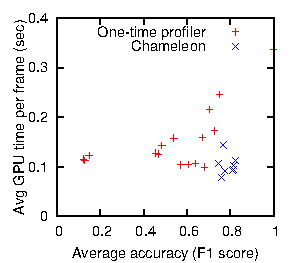
\includegraphics[width=0.33\textwidth]{PaperGraphs/PipeLineA_Smoothed_Location_true_Tradeoff.pdf}
        \label{subfig:1}
    }\\
    \subfloat[]
    {
        \includegraphics[width=0.33\textwidth]{PaperGraphs/PipeLineA_Smoothed_Location_false_AccThresh_0.8.pdf}
        \label{subfig:1}
    }
    \subfloat[]
    {
        \includegraphics[width=0.33\textwidth]{PaperGraphs/PipeLineA_Smoothed_Location_false_AccThresh_0.9.pdf}
        \label{subfig:1}
    }
    \subfloat[]
    {
        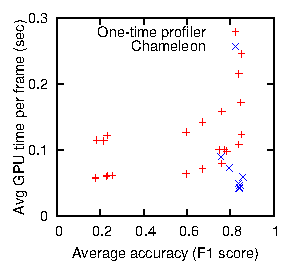
\includegraphics[width=0.33\textwidth]{PaperGraphs/PipeLineA_Smoothed_Location_false_Tradeoff.pdf}
        \label{subfig:1}
    }
    \caption{Pipeline A}
    \label{fig:potential}
\end{figure*}

\begin{figure*}[t!]
    \centering
    \hspace{-0.5cm}
    \subfloat[]
    {
        \includegraphics[width=0.33\textwidth]{PaperGraphs/PipeLineA_Smoothed_Locatiofalse_AccThresh_0.8.pdf}
        \label{subfig:1}
    }
    \subfloat[]
    {
        \includegraphics[width=0.33\textwidth]{PaperGraphs/PipeLineA_Smoothed_Location_false_AccThresh_0.9.pdf}
        \label{subfig:1}
    }
    \subfloat[]
    {
        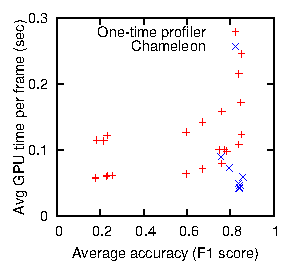
\includegraphics[width=0.33\textwidth]{PaperGraphs/PipeLineA_Smoothed_Location_false_Tradeoff.pdf}
        \label{subfig:1}
    }
    \caption{Pipeline B}
    \label{fig:potential}
\end{figure*}


\subsection{Impact of cross-video inference}

\subsection{Impact of temporal incremental updates}

\subsection{Impact of reducing configuration spaces}